 \documentclass[9pt]{beamer}
%\documentclass[compress,9pt,usenames,dvipsnames]{beamer}
% \usepackage[utf8]{inputenc}
% \includeonlyframes{current}
\usepackage{dbt}
\setbeamercovered{dynamic}
\usepackage{etex}
\usepackage{graphicx,url,psfrag}
\usepackage{tikz}
\usetikzlibrary{decorations.pathreplacing,calc,decorations.fractals,through,shapes,patterns,arrows.meta,decorations.pathreplacing,arrows,shapes}
% \usepackage[center]{subfigure}
\usepackage{enumerate}
\usepackage[makeroom]{cancel}
\usepackage{mathtools}
\usepackage{graphbox}
\usepackage{amssymb}
\usepackage{comment}
\excludecomment{codes}
% \usepackage{movie15}
% \usepackage[showframe]{geometry}
% \usepackage{enumitem}
\usepackage{pdfpages}

%
% for warning sign
%
\usepackage{pgfplots}
\usepackage{stackengine}
\usepackage{scalerel}
\usepackage{xcolor}
\newcommand\dangersign[1][2ex]{%
  \renewcommand\stacktype{L}%
  \scaleto{\stackon[1.3pt]{\color{red}$\triangle$}{\tiny !}}{#1}%
}
% %  The following is to show codes:
\usepackage{listings}
% \usepackage{color}

\usepackage{poker}
\setkeys{poker}{inline=symbol}
\usepackage{epsdice}

\definecolor{dkgreen}{rgb}{0,0.6,0}
\definecolor{gray}{rgb}{0.5,0.5,0.5}
\definecolor{mauve}{rgb}{0.58,0,0.82}

\lstset{frame=tb,
  language=Java,
  aboveskip=3mm,
  belowskip=3mm,
  showstringspaces=false,
  columns=flexible,
  basicstyle={\small\ttfamily},
  numbers=none,
  numberstyle=\tiny\color{gray},
  keywordstyle=\color{blue},
  commentstyle=\color{dkgreen},
  stringstyle=\color{mauve},
  breaklines=true,
  breakatwhitespace=true,
  tabsize=3
}
\lstset{language=Python}

\lstset{ %
  language=Python,                     % the language of the code
  basicstyle=\footnotesize,       % the size of the fonts that are used for the code
  numbers=left,                   % where to put the line-numbers
  numberstyle=\tiny\color{gray},  % the style that is used for the line-numbers
  stepnumber=1,                   % the step between two line-numbers. If it's 1, each line
                                  % will be numbered
  numbersep=5pt,                  % how far the line-numbers are from the code
  backgroundcolor=\color{black},  % choose the background color. You must add \usepackage{color}
  showspaces=false,               % show spaces adding particular underscores
  showstringspaces=false,         % underline spaces within strings
  showtabs=false,                 % show tabs within strings adding particular underscores
  frame=single,                   % adds a frame around the code
  rulecolor=\color{black},        % if not set, the frame-color may be changed on line-breaks within not-black text (e.g. commens (green here))
  tabsize=2,                      % sets default tabsize to 2 spaces
  captionpos=b,                   % sets the caption-position to bottom
  breaklines=true,                % sets automatic line breaking
  breakatwhitespace=false,        % sets if automatic breaks should only happen at whitespace
  title=\lstname,                 % show the filename of files included with \lstinputlisting;
                                  % also try caption instead of title
  keywordstyle=\color{blue},      % keyword style
  commentstyle=\color{dkgreen},   % comment style
  stringstyle=\color{mauve},      % string literal style
  escapeinside={\%*}{*)},         % if you want to add a comment within your code
  morekeywords={*,...}            % if you want to add more keywords to the set
}
% \usepackage[usenames,dvipsnames]{color}
% \lstset{
%   language=R,                     % the language of the code
%   basicstyle=\tiny\ttfamily, % the size of the fonts that are used for the code
%   numbers=left,                   % where to put the line-numbers
%   numberstyle=\tiny\color{Blue},  % the style that is used for the line-numbers
%   stepnumber=1,                   % the step between two line-numbers. If it is 1, each line
%                                   % will be numbered
%   numbersep=5pt,                  % how far the line-numbers are from the code
%   backgroundcolor=\color{white},  % choose the background color. You must add \usepackage{color}
%   showspaces=false,               % show spaces adding particular underscores
%   showstringspaces=false,         % underline spaces within strings
%   showtabs=false,                 % show tabs within strings adding particular underscores
%   frame=single,                   % adds a frame around the code
%   rulecolor=\color{black},        % if not set, the frame-color may be changed on line-breaks within not-black text (e.g. commens (green here))
%   tabsize=2,                      % sets default tabsize to 2 spaces
%   captionpos=b,                   % sets the caption-position to bottom
%   breaklines=true,                % sets automatic line breaking
%   breakatwhitespace=false,        % sets if automatic breaks should only happen at whitespace
%   keywordstyle=\color{RoyalBlue},      % keyword style
%   commentstyle=\color{YellowGreen},   % comment style
%   stringstyle=\color{ForestGreen}      % string literal style
% }

% \usepackage[dvipsnames]{xcolor}
% \newcommand{\Cross}{\mathbin{\tikz [x=1.4ex,y=1.4ex,line width=.2ex] \draw (0,0) -- (1,1) (0,1) -- (1,0);}}%
\newcommand{\Crossme}[1]{\!\!
\tikz [black,x=1.1em,y=1.1em,line width=.4ex]
\draw (-0.5,-0.5) -- (0,0) node {\footnotesize #1} -- (0.5,0.5) (0.5,-0.5) -- (-0.5,0.5);}%
\newcommand{\Checkme}[1]{\!\!
\tikz [x=1.1em,y=1.1em,line width=.4ex]
\draw [black] (0,0.7) -- (0.3,0) --(0.9,1.0) (0.5,0.5) node {\footnotesize #1};}
% \beamerdefaultoverlayspecification{<+-| alert@+>} %(this will show line by line)
\beamerdefaultoverlayspecification{<+->} %(this will show line by

% \usepackage{natbib}
% \input{../myMathSymbols.tex}
% \newcommand{\tlMr}[4]{\:{}^{\hspace{0.2em}#1}_{#2} \hspace{-0.1em}#3_{#4}}

% Smiley face\Smiley{} \Frowny{}
\usepackage{marvosym}
% -------------------------------------------------
%  Set directory for figs
% -------------------------------------------------
\usepackage{grffile}
\graphicspath{{Codes/}}
% -------------------------------------------------
%  Define colors
% -------------------------------------------------
\def\refcolor{cyan}
\def\excolor{brown}
% \usepackage{color}
% \usepackage[dvipsnames]{xcolor}


% % % Define danger sign
\newcommand*{\TakeFourierOrnament}[1]{{%
\fontencoding{U}\fontfamily{futs}\selectfont\char#1}}
\newcommand*{\danger}{\TakeFourierOrnament{66}}


% -------------------------------------------------
%  Define short-hand symbols.
% -------------------------------------------------
\newcommand{\B}{\textbf{B}}
\newcommand{\PP}{\mathbb{P}}
\newcommand{\E}{\mathbb{E}}
\newcommand{\D}{\mathbb{D}}
\newcommand{\W}{\dot{W}}
\newcommand{\ud}{\ensuremath{\mathrm{d}}}
\newcommand{\Ceil}[1]{\left\lceil #1 \right\rceil}
\newcommand{\Floor}[1]{\left\lfloor #1 \right\rfloor}
\newcommand{\sgn}{\text{sgn}}
\newcommand{\Lad}{\text{L}_{\text{ad}}^2}
\newcommand{\SIB}[2]{\mathcal{I}_{#2}\left[#1 \right]}
\newcommand{\Indt}[1]{1_{\left\{#1 \right\}}}
\newcommand{\LadInPrd}[1]{\left\langle #1 \right\rangle_{\text{L}_\text{ad}^2}}
\newcommand{\LadNorm}[1]{\left|\left|  #1 \right|\right|_{\text{L}_\text{ad}^2}}
\newcommand{\Norm}[1]{\left|\left|  #1   \right|\right|}
\newcommand{\Ito}{It\^{o} }
\newcommand{\Itos}{It\^{o}'s }
\newcommand{\spt}[1]{\text{supp}\left(#1\right)}
\newcommand{\InPrd}[1]{\left\langle #1 \right\rangle}
\newcommand{\mr}{\textbf{r}}
\newcommand{\Ei}{\text{Ei}}
\newcommand{\arctanh}{\operatorname{arctanh}}
\newcommand{\ind}[1]{\mathbb{I}_{\left\{ {#1} \right\} }}
\newcommand{\Var}{\text{Var}}
\newcommand{\Cov}{\text{Cov}}
\newcommand{\Corr}{\text{Corr}}

\newcommand{\baseurl}[1]{\footnotesize\url{http://math.emory.edu/~lchen41/teaching/2020_Spring/#1}}


\newcommand*\mystrut[1]{\vrule width0pt height0pt depth#1\relax} % adding vertical space

\DeclareMathOperator{\esssup}{\ensuremath{ess\,sup}}

\newcommand{\steps}[1]{\vskip 0.3cm \textbf{#1}}
\newcommand{\calB}{\mathcal{B}}
\newcommand{\calC}{\mathcal{C}}
\newcommand{\calD}{\mathcal{D}}
\newcommand{\calE}{\mathcal{E}}
\newcommand{\calF}{\mathcal{F}}
\newcommand{\calG}{\mathcal{G}}
\newcommand{\calK}{\mathcal{K}}
\newcommand{\calH}{\mathcal{H}}
\newcommand{\calI}{\mathcal{I}}
\newcommand{\calL}{\mathcal{L}}
\newcommand{\calM}{\mathcal{M}}
\newcommand{\calN}{\mathcal{N}}
\newcommand{\calO}{\mathcal{O}}
\newcommand{\calT}{\mathcal{T}}
\newcommand{\calP}{\mathcal{P}}
\newcommand{\calR}{\mathcal{R}}
\newcommand{\calS}{\mathcal{S}}
\newcommand{\calV}{\mathcal{V}}
\newcommand{\bbC}{\mathbb{C}}
\newcommand{\bbN}{\mathbb{N}}
\newcommand{\bbP}{\mathbb{P}}
\newcommand{\bbZ}{\mathbb{Z}}
\newcommand{\myVec}[1]{\overrightarrow{#1}}
\newcommand{\sincos}{\begin{array}{c} \cos \\ \sin \end{array}\!\!}
\newcommand{\CvBc}[1]{\left\{\:#1\:\right\}}
\newcommand*{\one}{{{\rm 1\mkern-1.5mu}\!{\rm I}}}

\newcommand{\OneFrame}[1]{
\begin{enumerate}\item[#1] \phantom{av} \\[20em]\vfill\phantom{av}\myEnd\end{enumerate}}

\newcommand{\bH}{\ensuremath{\mathrm{H}}}
\newcommand{\Ai}{\ensuremath{\mathrm{Ai}}}

\newcommand{\R}{\mathbb{R}}
\newcommand{\myEnd}{\hfill$\square$}
\newcommand{\ds}{\displaystyle}
\newcommand{\Shi}{\text{Shi}}
\newcommand{\Chi}{\text{Chi}}
\newcommand{\Erf}{\ensuremath{\mathrm{erf}}}
\newcommand{\Erfc}{\ensuremath{\mathrm{erfc}}}
\newcommand{\He}{\ensuremath{\mathrm{He}}}
\newcommand{\Res}{\ensuremath{\mathrm{Res}}}

\newcommand{\mySeparateLine}{\begin{center}
 \makebox[\linewidth]{\rule{0.6\paperwidth}{0.4pt}}
\end{center}}

\theoremstyle{definition}
% \newtheorem{definition}[theorem]{Definition}
% \newtheorem{hypothesis}[theorem]{Hypothesis}
\newtheorem{assumption}[theorem]{Assumption}

\theoremstyle{plain}
% \newtheorem{theorem}{Theorem}
% \newtheorem{corollary}[theorem]{Corollary}
% \newtheorem{lemma}[theorem]{Lemma}
\newtheorem{proposition}[theorem]{Proposition}

\mode<presentation>
{
%      \usetheme{Warsaw}
%     \usetheme{JuanLesPins}
%  \usetheme{Hannover}
%  \usetheme{Montpellier}
   \useoutertheme{default}
  % or ...

  \setbeamercovered{transparent}
  % or whatever (possibly just delete it)
 \setbeamertemplate{frametitle}{
  \begin{centering}
    \color{blue}
    {\insertframetitle}
    \par
  \end{centering}
  }
}
\usefoottemplate{\hfill \insertframenumber{}}
% \inserttotalframenumber

\usepackage[english]{babel}
% or whatever

% \usepackage[latin1]{inputenc}
% or whatever

\usepackage{times}
\usepackage[T1]{fontenc}
% Or whatever. Note that the encoding and the font should match. If T1
% does not look nice, try deleting the line with the fontenc.

% \DeclareMathOperator{\Lip}{Lip}
\DeclareMathOperator{\lip}{l}
% \DeclareMathOperator{\Vip}{\overline{v}}
% \DeclareMathOperator{\vip}{\underline{v}}
% \DeclareMathOperator{\vv}{v}
% \DeclareMathOperator{\BC}{BC}
% \DeclareMathOperator{\CH}{CD}

\usepackage{pgfpages}
% \setbeameroption{show notes}
% \setbeamertemplate{note page}[plain]
% \setbeameroption{second mode text on second screen=right}
% \setbeameroption{show notes on second screen=right}
%

% Delete this, if you do not want the table of contents to pop up at
% the beginning of each subsection:
% \AtBeginSubsection[]
% {
%   \begin{frame}<beamer>{Outline}
%     \tableofcontents[currentsection,currentsubsection]
%   \end{frame}
% }

% If you wish to uncover everything in a step-wise fashion, uncomment
% the following command:
% \beamerdefaultoverlayspecification{<+->}

% % % % % % % % % % % % % % % % % % %
%  Define a block
% % % % % % % % % % % % % % % % % % %
\newenvironment<>{problock}[1]{%
  \begin{actionenv}#2%
      \def\insertblocktitle{#1}%
      \par%
      \mode<presentation>{%
        \setbeamercolor{block title}{fg=white,bg=olive!95!black}
       \setbeamercolor{block body}{fg=black,bg=olive!25!white}
       \setbeamercolor{itemize item}{fg=white!20!white}
       \setbeamertemplate{itemize item}[triangle]
     }%
      \usebeamertemplate{block begin}}
    {\par\usebeamertemplate{block end}\end{actionenv}}

\newenvironment<>{assblock}[1]{%
  \begin{actionenv}#2%
      \def\insertblocktitle{#1}%
      \par%
      \mode<presentation>{%
        \setbeamercolor{block title}{fg=white,bg=green!50!black}
       \setbeamercolor{block body}{fg=black,bg=green!10}
       \setbeamercolor{itemize item}{fg=green!80!black}
       \setbeamertemplate{itemize item}[triangle]
     }%
      \usebeamertemplate{block begin}}
    {\par\usebeamertemplate{block end}\end{actionenv}}


% \newtheorem{proofnoend}{Proof.}
% \AtBeginEnvironment{proofnoend}{%
%   \setbeamercolor{block title}{use=example text,fg=lgtblue,bg=background}
%   % \setbeamercolor{block body}{parent=normal text,use=block title example,fg=yellow}
% }

% Define some colors
\definecolor{white}{HTML}{FFFFFF}              % #FFFFFF
\definecolor{pink}{HTML}{FB73BE}               % #FB73BE
\definecolor{coral}{HTML}{FF8D71}              % #FF8D71
\definecolor{yellow}{HTML}{FFE066}             % #FFE066
\definecolor{teal}{HTML}{59F3CE}               % #59F3CE
\definecolor{lgtblue}{HTML}{65D0FA} 	       % #65D0FA
\definecolor{blue}{HTML}{4984F2}               % #4984F2
\definecolor{purple}{HTML}{A87DFF}             % #A87DFF
\definecolor{red}{HTML}{FF3d30}                % #FF3d30
% \definecolor{magenta}{HTML}{FF80FF}                % #FF3d30
\definecolor{green}{HTML}{BBFFB9}              % #BBFFB9
% \definecolor{green}{HTML}{59F3CE}              % #BBFFB9
\setbeamercolor{alerted text}{fg=red}
% \setbeamercolor{block title}{bg=background,fg=lgtblue}

\setbeamercolor{section in toc}{fg=yellow}
\setbeamercolor{subsection in toc}{fg=red}

% \newtheorem{myexample}{\it Example}[section]
\newcounter{myexample}[section]
\resetcounteronoverlays{myexample}
\newenvironment{myexample}[1][]{\refstepcounter{myexample}\par\medskip
\noindent \textbf{\textcolor{green}{Example~\mySecNum-\themyexample~#1}} \rmfamily}{\medskip}

\newcounter{mydefinition}[section]
\resetcounteronoverlays{mydefinition}
\newenvironment{mydefinition}[1][]{\refstepcounter{mydefinition}\par\medskip
\noindent \textbf{\textcolor{yellow}{Definition~\mySecNum-\themydefinition~#1}} \rmfamily}{\medskip}

% \NewCommandCopy{\oldref}{\ref}
% \let\oldref\ref
\newcommand{\myref}[1]{\mySecNum-\ref{#1}}

\newcounter{remark}[section]
\resetcounteronoverlays{remark}
\newenvironment{remark}[1][]{\refstepcounter{remark}\par\medskip
\noindent \textbf{\textcolor{blue}{Remark~\mySecNum-\theremark~#1}} \rmfamily}{\medskip}

\newcounter{mythm}[section]
\resetcounteronoverlays{mythm}
\newenvironment{mythm}[1][]{\refstepcounter{mythm}\par\medskip
\noindent \textbf{\textcolor{lgtblue}{Theorem~\mySecNum-\themythm~#1}} \rmfamily}{\medskip}

\newenvironment{mycor}[1][]{\refstepcounter{mythm}\par\medskip
\noindent \textbf{\textcolor{lgtblue}{Corollary~\mySecNum-\themythm~#1}} \rmfamily}{\medskip}

% \newtheorem{solution}{\textcolor{purple}{Solution}}
\newenvironment{mysol}[1][]{\par\medskip
\noindent \textbf{\textcolor{purple}{Solution#1.~}} \rmfamily}{\medskip}

\long\def\script#1{}

\usepackage{etoolbox}
\usepackage{ifthen}

% Put this file into the preamble and call it via
% \input{tikzdice.tex}
%
% Jesse Hamner
% https://github.com/jessehamner/tikzdice
% 2020


\usetikzlibrary{arrows}

\tikzset{
  treenode/.style = {align=center, text centered,
    font=\sffamily},
  arn_n/.style = {treenode, font=\sffamily\bfseries, draw=black,
    fill=black, text width=1.5em},
  arn_r/.style = {treenode, text width=1.5em},
  arn_x/.style = {treenode, minimum width=0.5em, minimum height=0.5em}
}

\newcommand{\majelaxis}{0.5}
\newcommand{\minelaxis}{0.125}

\newcommand{\headtext}{\color{red}\textbf{H}}

\newcommand{\dieone}{\maindie{1}{0}}
\newcommand{\dietwo}{\maindie{2}{0}}
\newcommand{\diethree}{\maindie{3}{0}}
\newcommand{\diefour}{\maindie{4}{0}}
\newcommand{\diefive}{\maindie{5}{0}}
\newcommand{\diesix}{\maindie{6}{0}}

\newcommand{\pipsize}{3.05pt}
\newcommand{\diecolor}{red}
\newcommand{\pipcolor}{red}
\newcommand{\fieldfill}{white}

\newcommand{\piplocation}[2]{\filldraw[fill=\pipcolor] (#1,#2) circle (\pipsize);}

\newcommand{\piplocationone}{\piplocation{0.25}{0.25}}
\newcommand{\piplocationtwo}{\piplocation{0.50}{0.25}}
\newcommand{\piplocationthree}{\piplocation{0.75}{0.25}}
\newcommand{\piplocationfour}{\piplocation{0.25}{0.50}}
\newcommand{\piplocationfive}{\piplocation{0.50}{0.50}}
\newcommand{\piplocationsix}{\piplocation{0.75}{0.50}}
\newcommand{\piplocationseven}{\piplocation{0.25}{0.75}}
\newcommand{\piplocationeight}{\piplocation{0.50}{0.75}}
\newcommand{\piplocationnine}{\piplocation{0.75}{0.75}}

\newcommand{\spreadsix}{\piplocation{0.20}{0.20}\piplocation{0.20}{0.80}
						\piplocation{0.80}{0.20}\piplocation{0.80}{0.80}
						\piplocation{0.50}{0.20}\piplocation{0.50}{0.80}}

\newcommand{\maindie}[2]{
\ifthenelse{#2 = 0}{\renewcommand{\diecolor}{black}\renewcommand{\pipcolor}{black}\renewcommand{\fieldfill}{white}}{}%
\ifthenelse{#2 = 1}{\renewcommand{\diecolor}{red}\renewcommand{\pipcolor}{red}\renewcommand{\fieldfill}{white}}{}%
\ifthenelse{#2 = 2}{\renewcommand{\diecolor}{blue}\renewcommand{\pipcolor}{blue}\renewcommand{\fieldfill}{white}}{}%
\ifthenelse{#2 = 3}{\renewcommand{\diecolor}{black}\renewcommand{\pipcolor}{white}\renewcommand{\fieldfill}{black}}{}%
\begin{tikzpicture}
  \draw[very thick, rounded corners, \diecolor, fill=\fieldfill] (0,0) rectangle (1,1);
  \ifthenelse{#1 = 1}{\piplocationfive}{}%
  \ifthenelse{#1 = 2}{\piplocationone\piplocationnine}{}%
  \ifthenelse{#1 = 3}{\piplocationone\piplocationfive\piplocationnine}{}%
  \ifthenelse{#1 = 4}{\piplocationone\piplocationnine\piplocationthree\piplocationseven}{}%
  \ifthenelse{#1 = 5}{\piplocationone\piplocationnine\piplocationthree\piplocationseven\piplocationfive}{}%
  \ifthenelse{#1 = 6}{\piplocation{0.20}{0.25}\piplocation{0.20}{0.75}
					  \piplocation{0.80}{0.25}\piplocation{0.80}{0.75}
					  \piplocation{0.20}{0.50}\piplocation{0.80}{0.50}}{}%

  \ifthenelse{#1 = 7}{\spreadsix\piplocationfive}{}%
  \ifthenelse{#1 = 8}{\spreadsix\piplocation{0.20}{0.50}\piplocation{0.80}{0.50}}{}%
  \ifthenelse{#1 = 9}{\spreadsix\piplocation{0.20}{0.50}\piplocation{0.80}{0.50}\piplocationfive}{}%
  \ifthenelse{#1 = 0}{}{}%
%    \ifthenelse{#1 = 0}{\draw[very thick, rounded corners, \diecolor, fill=\diecolor!20] (0,0) rectangle (1,1);}{}%

\end{tikzpicture}
}


\pgfmathdeclarefunction{addone}{1}{
  \pgfmathparse{#1 + \majelaxis}
}

\pgfmathdeclarefunction{addtwo}{1}{
  \pgfmathparse{#1 + \majelaxis + \majelaxis}
}

\pgfmathdeclarefunction{addspace}{1}{
  \pgfmathparse{#1 + 1.15}
}


\newcommand{\coin}[4]{
  \pgfmathsetmacro{\argthree}{addone(#1)}
  \pgfmathsetmacro{\argtwo}{addtwo(#1)}

  \shade[left color=white, right color=black]
    ({\argthree},0mm) ellipse (\majelaxis cm and \minelaxis cm);
  \shade[left color=white, right color=black]
    ({#1},0mm) rectangle (\argtwo cm, 1mm);

  \draw({\argthree},0.5cm) node[color=blue, above]{#2};

  \draw[fill=#4]({\argthree},1mm) ellipse (\majelaxis cm and \minelaxis cm);
  \draw ({#1},0mm) arc (180:360:\majelaxis cm and \minelaxis cm);
  \draw({#1},0mm) -- ({#1}, 1mm);
  \draw({\argtwo},0mm) -- ({\argtwo}, 1mm);

  \draw({\argthree},-0.4cm) node[color=black, below]{#3};
}

\newcommand{\heads}[2]{
\coin{#1}{#2}{\headtext}{blue!50}
}

\newcommand{\tails}[2]{
\coin{#1}{#2}{{\color{gray!70}T}}{white}
}




\newcommand{\wtf}{\theheadpos & \makecoinrow{} \\}

\newcommand{\whichheads}{1}
\newcounter{num}
\setcounter{num}{1}
\newcounter{headpos}
\setcounter{headpos}{1}
\newcounter{int}
\setcounter{int}{1}


% Row of coins, one head, slot #1.

\newcommand{\makecoinrow}{
  \setcounter{int}{1}

  \begin{tikzpicture}[]
    \newdimen\R
    \R=0cm

    \loop
      \ifthenelse{\value{int}=\value{headpos}}{\heads{\R}{}}{\tails{\R}{}}
      \pgfmathsetmacro{\R}{addspace(\R)}
      \stepcounter{int}
      \ifnum \value{int}<11
    \repeat

  \end{tikzpicture}

  \smallskip
}



% Definition of circles and square
\def\firstcircle{(0,0) circle (1.5cm)}
\def\secondcircle{(2,0) circle (1.5cm)}
\def\firstsquare{(-1.6,-1.6) rectangle (1.6,1.6)}


\def\missed{\LARGE\textbf{X}}
\def\target{\begin{tikzpicture}
  \draw[ultra thick, black, fill=blue!55] (0,0) circle(1cm);
  \draw[fill=red!70] (0,0) circle(0.73cm);
  \draw[fill=yellow] (0,0) circle(0.35cm) node{\small$\times$};
\end{tikzpicture}}

% Set colors
\colorlet{circle edge}{blue!50}
\colorlet{circle area}{blue!20}
\colorlet{rectangle edge}{blue!50}
\colorlet{rectangle area}{blue!20}

\tikzset{filled/.style={fill=circle area, draw=circle edge, thick},
    	 outline/.style={draw=circle edge, thick}
	    }
% This line makes makes theorems and boxed environments align incorrectly (vertically) in Beamer, I suggest that you remove it
% \setlength{\parskip}{5mm}

% This command is a nice shortcut in my opinion that makes the dice aligned vertically when they're used with text or in math mode.
% Possibly you want to use another (optional?) argument for the scalebox parameter to tune the size
\newcommand\vcdice[2]{\vcenter{\hbox{\scalebox{0.4}{\maindie{#1}{#2}}}}}



\def\missed{\LARGE\textbf{X}}
\def\target{\begin{tikzpicture}
  \draw[ultra thick, black, fill=blue!55] (0,0) circle(1cm);
  \draw[fill=red!70] (0,0) circle(0.73cm);
  \draw[fill=yellow] (0,0) circle(0.35cm) node{\small$\times$};
\end{tikzpicture}}

\tikzset{
  treenode/.style = {align=center, text centered, font=\sffamily},
  arn_n/.style = {treenode, font=\sffamily\bfseries, draw=black, fill=black},
  arn_r/.style = {treenode},
  arn_x/.style = {treenode}
}


% {{{ The following is for git information
\usepackage{gitinfo2}
% }}}

% If you have a file called "university-logo-filename.xxx", where xxx
% is a graphic format that can be processed by latex or pdflatex,
% resp., then you can add a logo as follows:

% \pgfdeclareimage[height=1cm]{Emory}{figs/Emory.png}


\title % (optional, use only with long paper titles)
{
  An Invitation to Probability
}

% \subtitle
% {Research Plan} % (optional)

\author{
  Le Chen\\
  {\small\url{lzc0090@auburn.edu}}\\[1em]
  \textcolor{gray}{\small (Creative Commons Zero 1.0)} \\[3em]
  {\small Science Center Auditorium}\\[1em]
  {\small 5:30pm -- 6:30pm, June 08, 2022}
}


\institute[Auburn University]{
 \textcolor{gray}{Github Hash:~\gitAbbrevHash} \\[1em]
 \textcolor{gray}{\gitCommitterIsoDate} \\[1em]
 {\tiny\textcolor{gray}{\url{https://github.com/chenle02/2012_Science_Summer_Institute_Auburn_Probability_by_Le}}}
 \vspace{5em}
}

\date[Auburn]{
  Summer Science Institute 2022\\
  Auburn University
}




\begin{document}
\begin{frame}[noframenumbering] \titlepage
\end{frame}
\begin{frame} \tableofcontents\end{frame}
\section{What is chance}%
\begin{frame}[fragile] % What is Chance?
\begin{center}
  \huge
  What is CHANCE?
\end{center}
\end{frame}
\begin{frame}[fragile,t] % Tyche
  \frametitle{{\it Tyche} -- The Greek goddess of chance}
  \begin{center}
    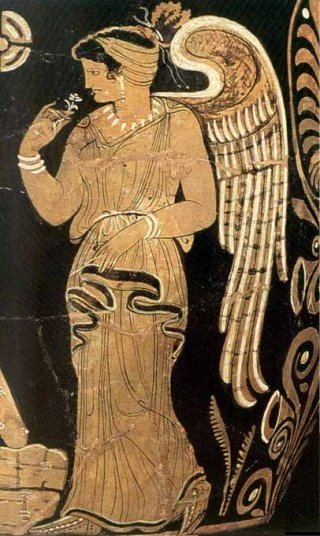
\includegraphics[scale=0.35]{./figs/Tyche.jpg} \quad
    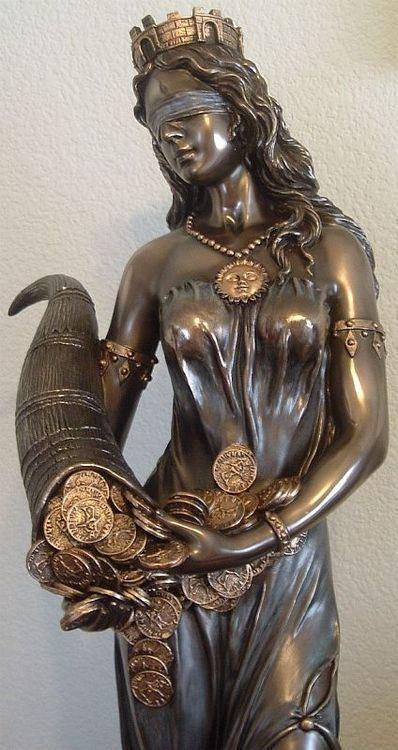
\includegraphics[scale=0.25]{./figs/Tyche2.jpg}
  \end{center}
\end{frame}
\begin{frame}[fragile] % Fortuna
  \frametitle{{\it Fortuna} -- The goddess of chance in Roman religion}
  \begin{center}
    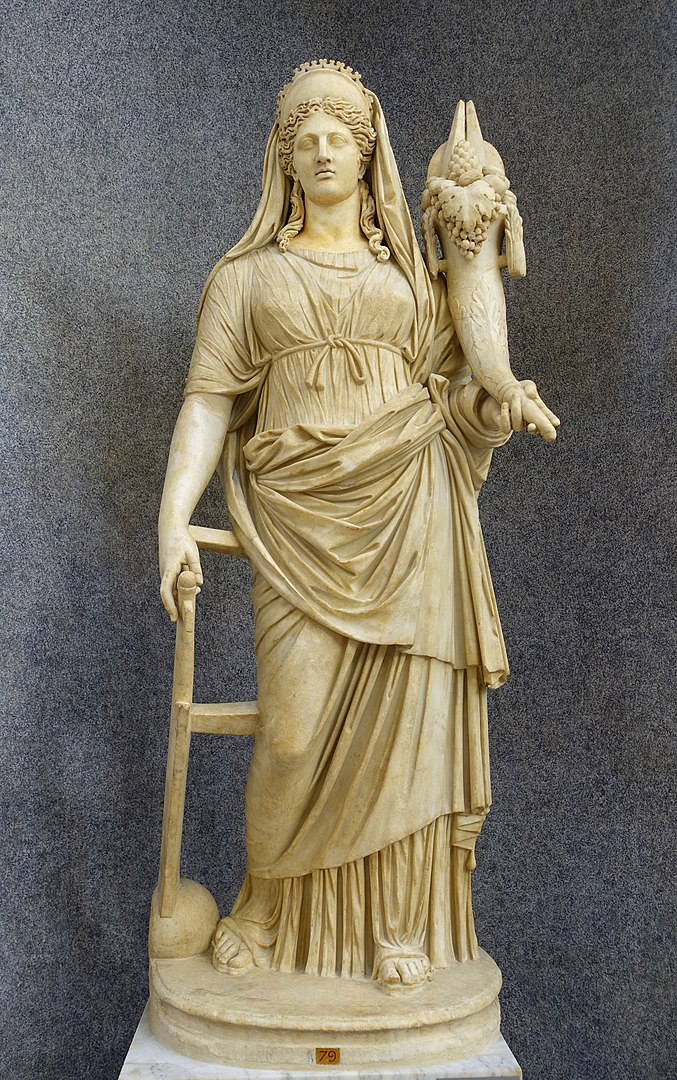
\includegraphics[scale=0.172]{./figs/Fortuna.jpg} \quad
    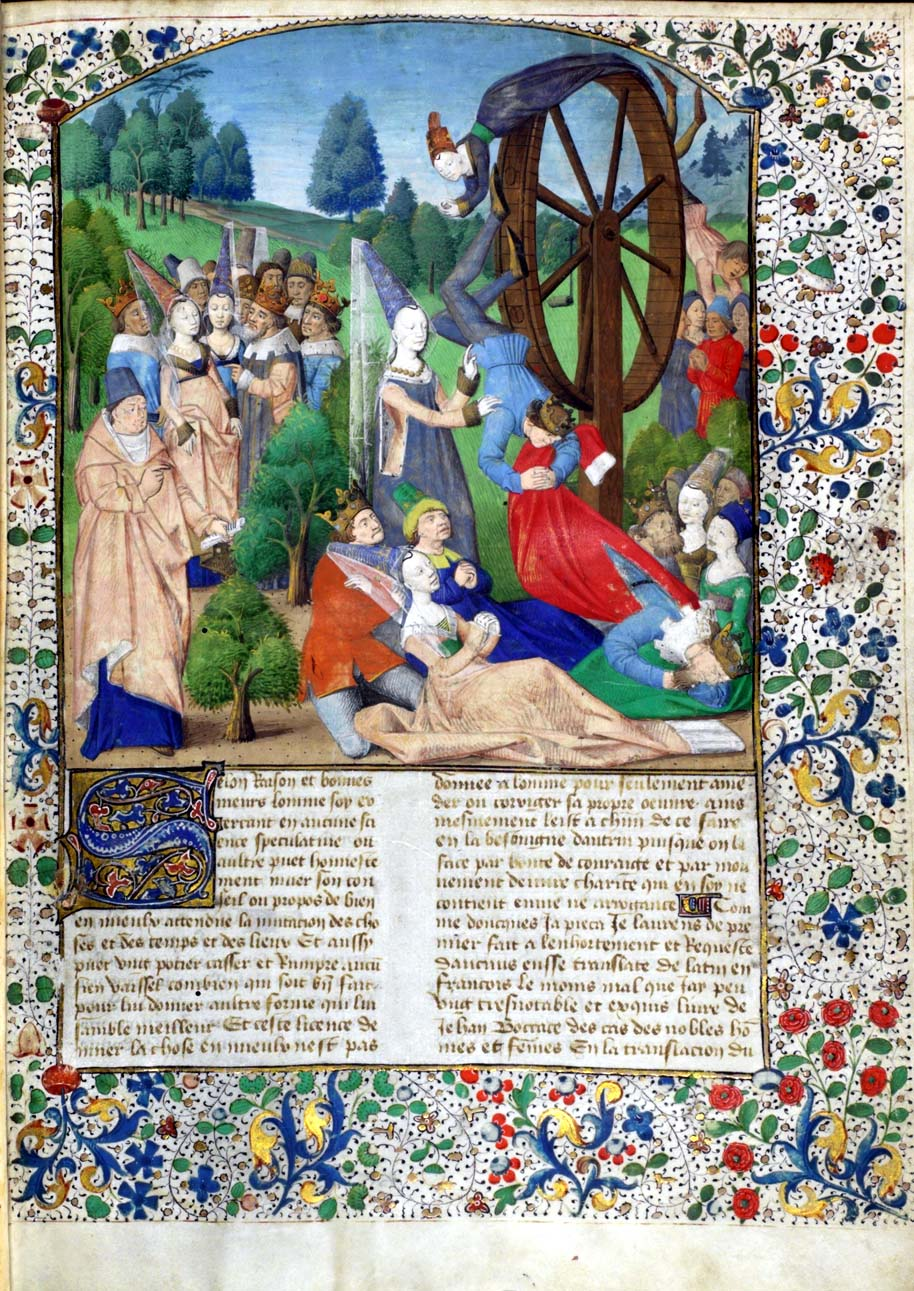
\includegraphics[scale=0.40]{./figs/ForutuneWheel.jpg}
  \end{center}
\end{frame}
\begin{frame}[fragile] % COMENTS
  \frametitle{{\it I Ching} in China ($\sim$ 6th century B.C.)}
 \begin{center}
   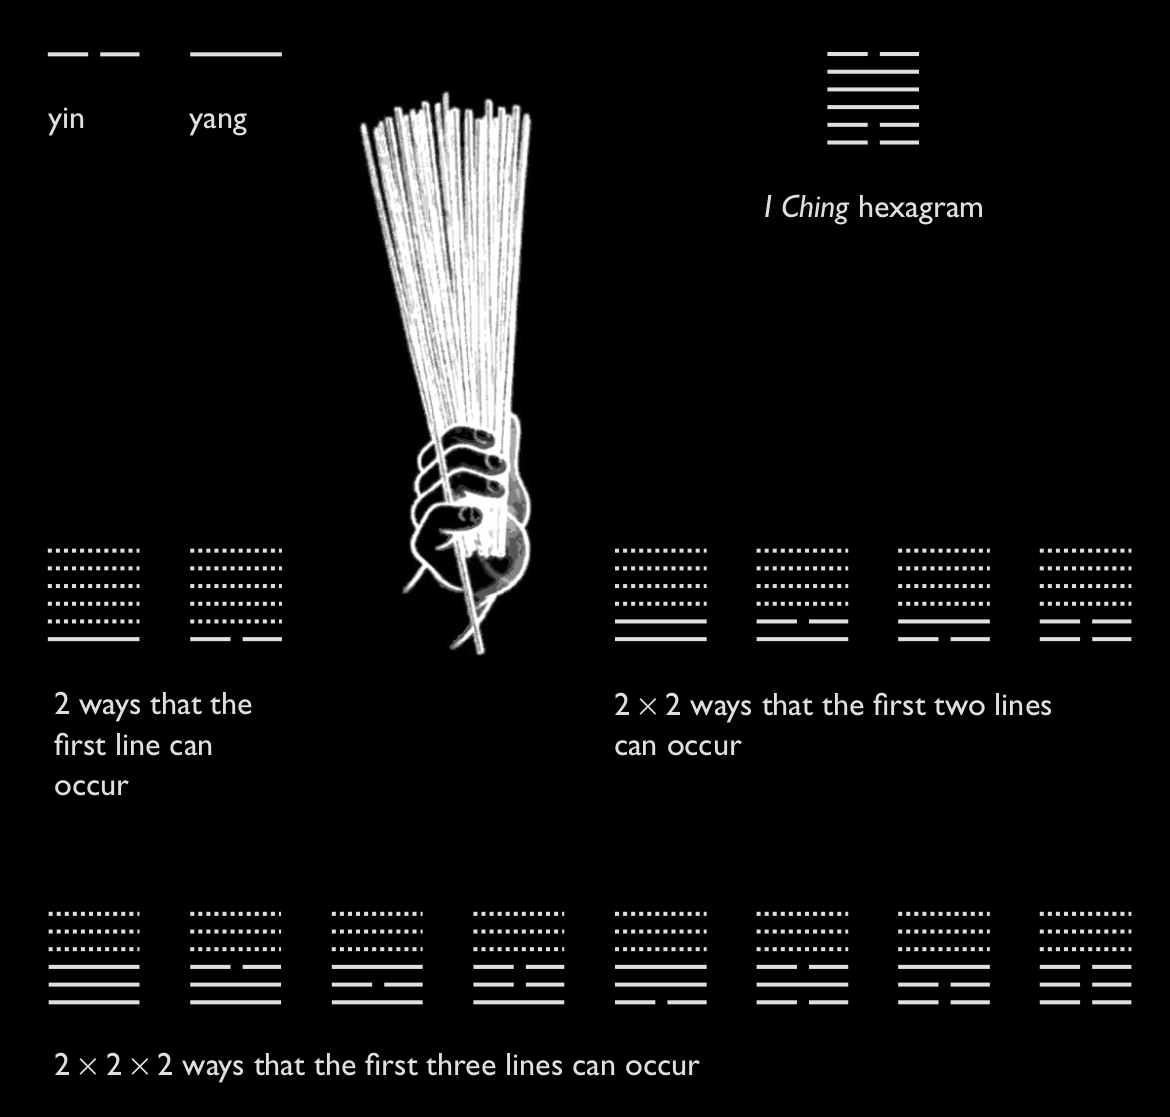
\includegraphics[scale=0.15]{./figs/IChing-neg.png}
   \footnote{Image is from Bennett (1998), {\it Randomness}, Harvard University Press.}
 \end{center}
\end{frame}
\begin{frame}[fragile] % Democritus
  \frametitle{{\it Democritus} (460 -- 370 BC) \\ --- Father of modern science}
  \begin{center}
    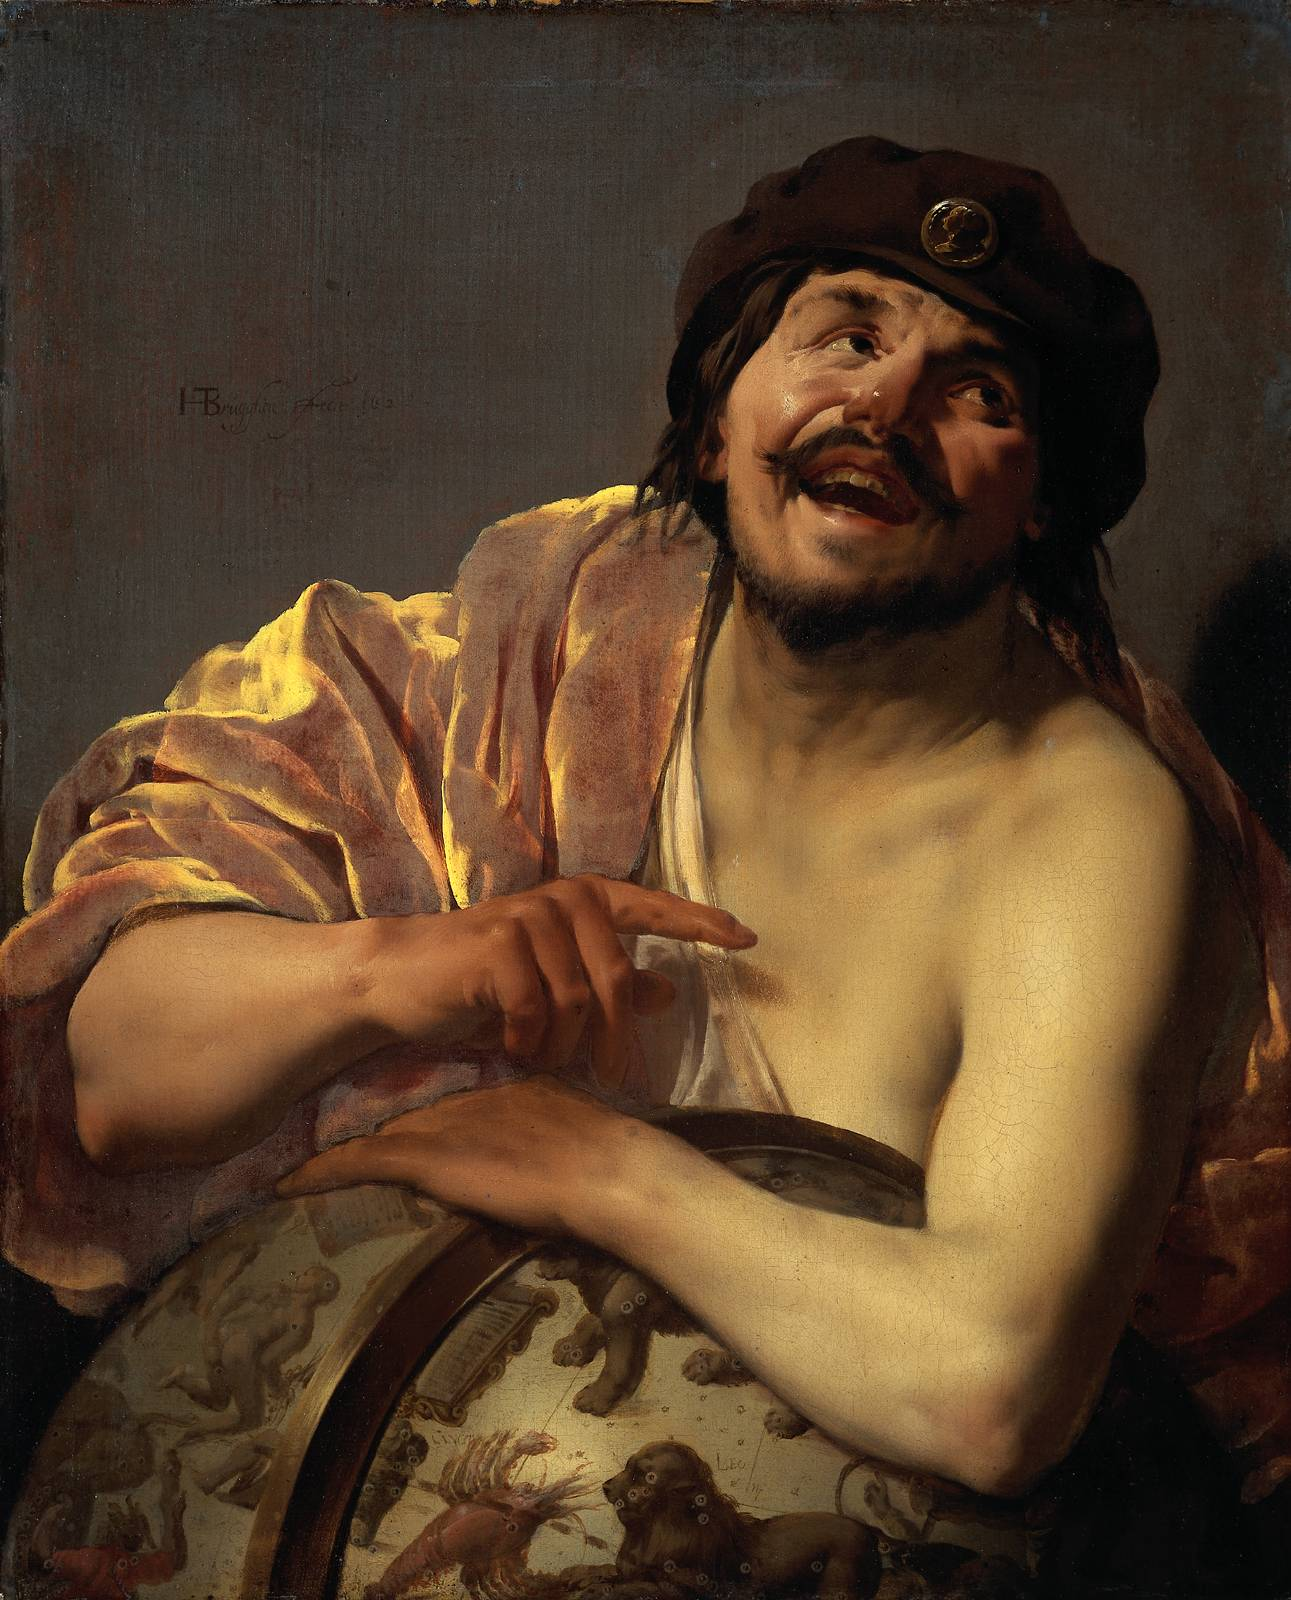
\includegraphics[scale=0.09]{./figs/Democritus.jpg} \qquad
    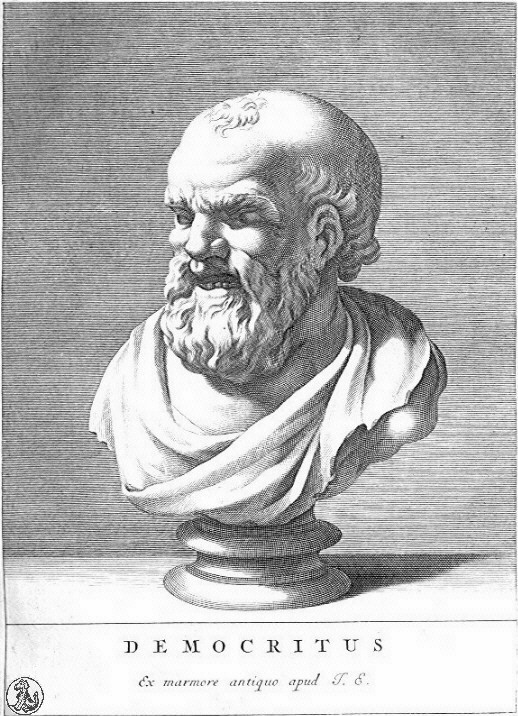
\includegraphics[scale=0.30]{./figs/Democritus2.jpg}
    \bigskip


    Atomic theory of the universe:\\ \bigskip

    A physical chance affecting all the atoms\\
    that made up the universe.
  \end{center}
\end{frame}
\begin{frame}[fragile] % Gamces of chance
  \frametitle{Games of chance \\ --- using knucklebones or dice}
  \begin{center}
    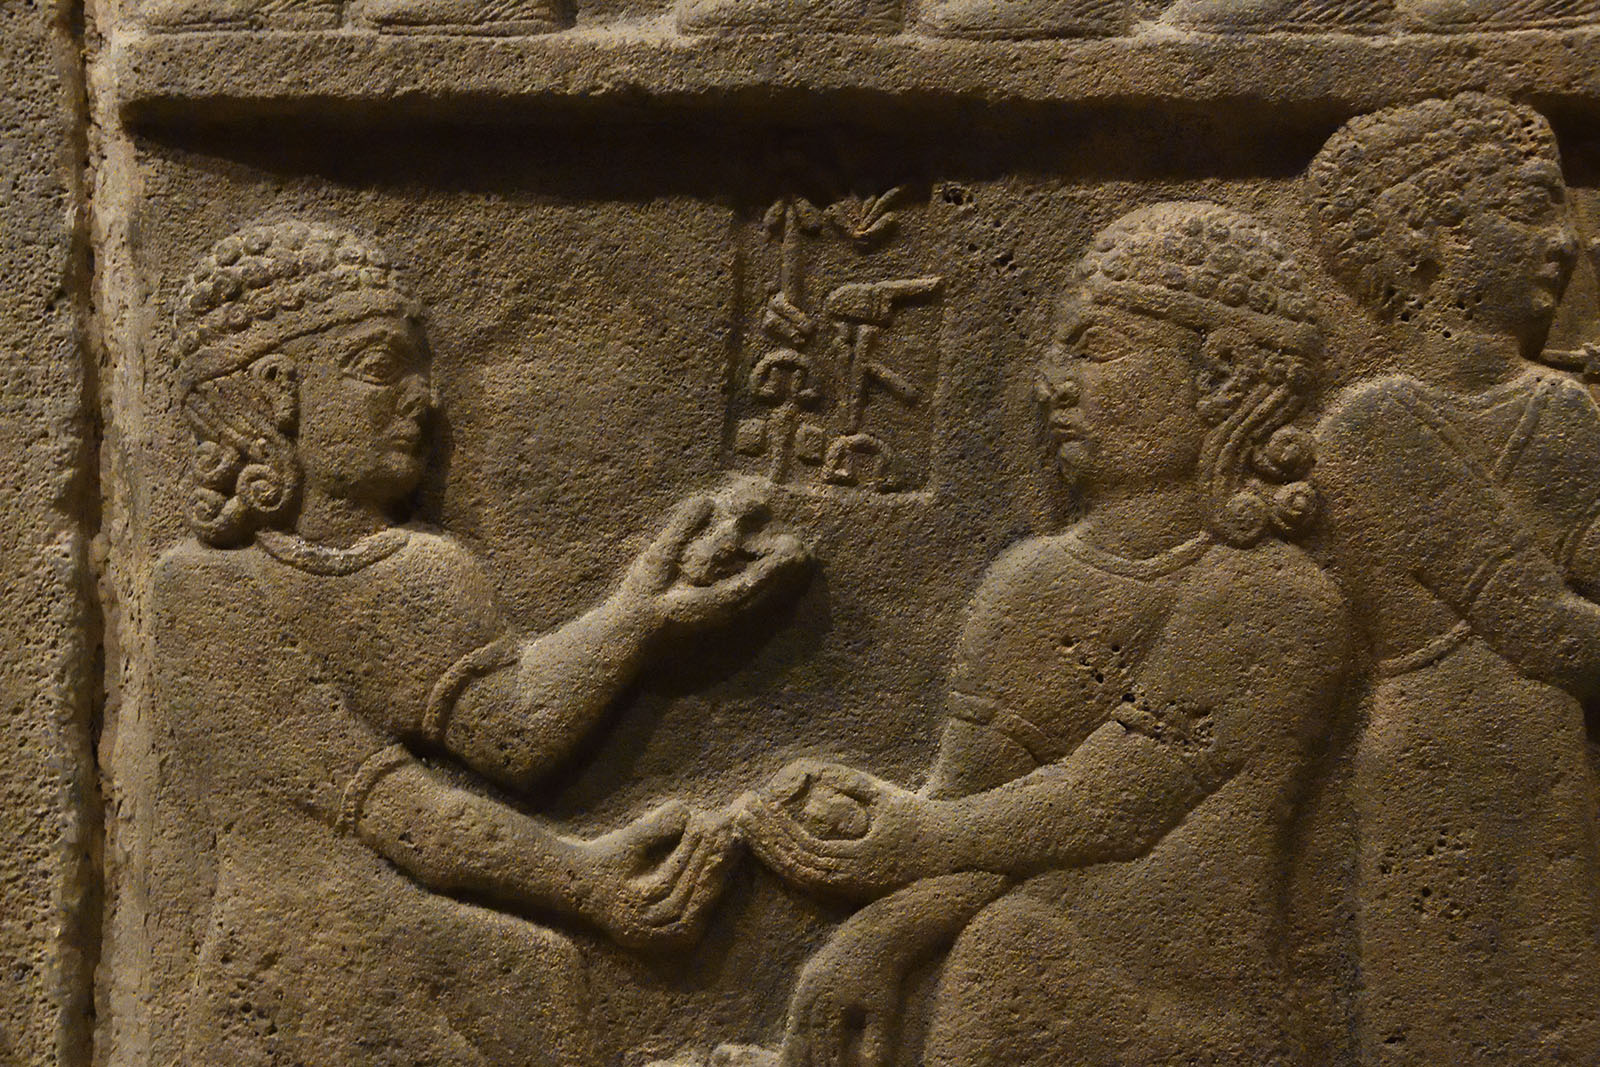
\includegraphics[scale=0.40]{./figs/Knucklebones2.jpg} \quad
    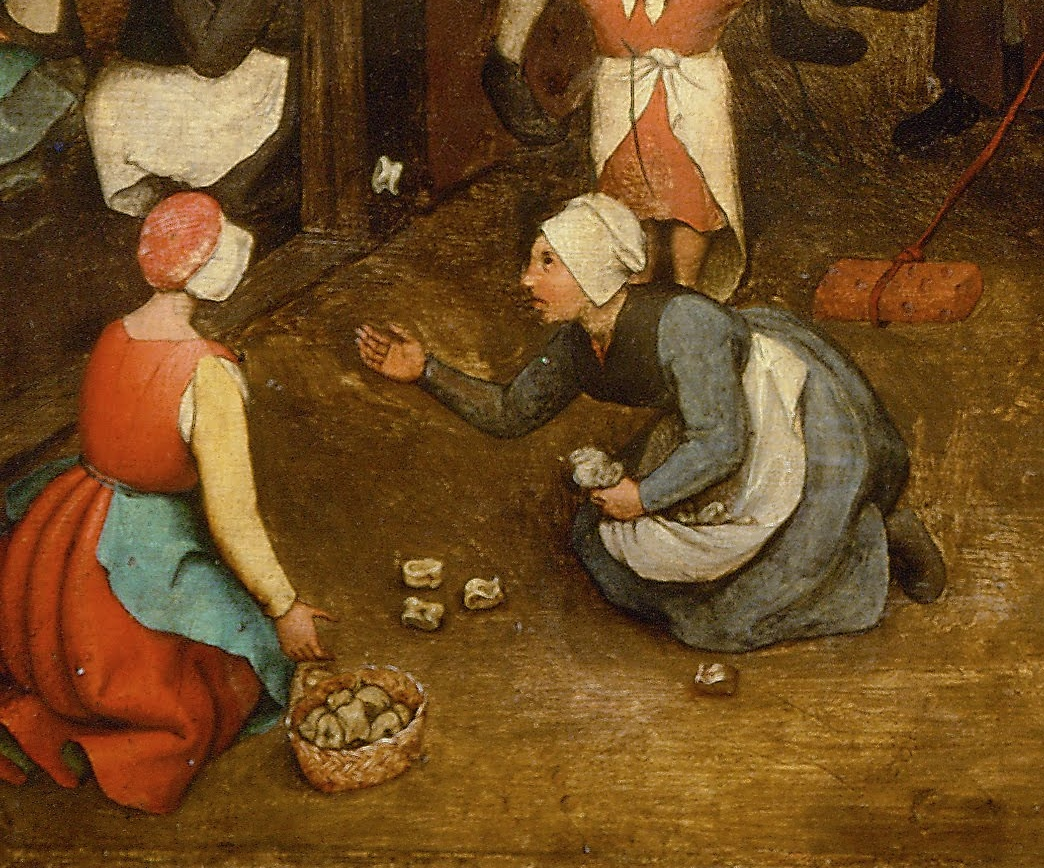
\includegraphics[scale=0.172]{./figs/Knucklebones.jpg}
    \bigskip

    Known to Egyptians, Babylonians, Romans, ...
  \end{center}
\end{frame}
\begin{frame}[fragile] % Conclude -- No theory
 \begin{center}
   There was no qualitative theory of chance in these times.
 \end{center}
\end{frame}
\section{How to measure chance}%
\begin{frame}[fragile] % Question posed
 \begin{center}
  \huge
  How to measure chance?
 \end{center}
\end{frame}
\begin{frame}[fragile,t] % Measure length
  \frametitle{How about measure length?}
  \begin{center}
    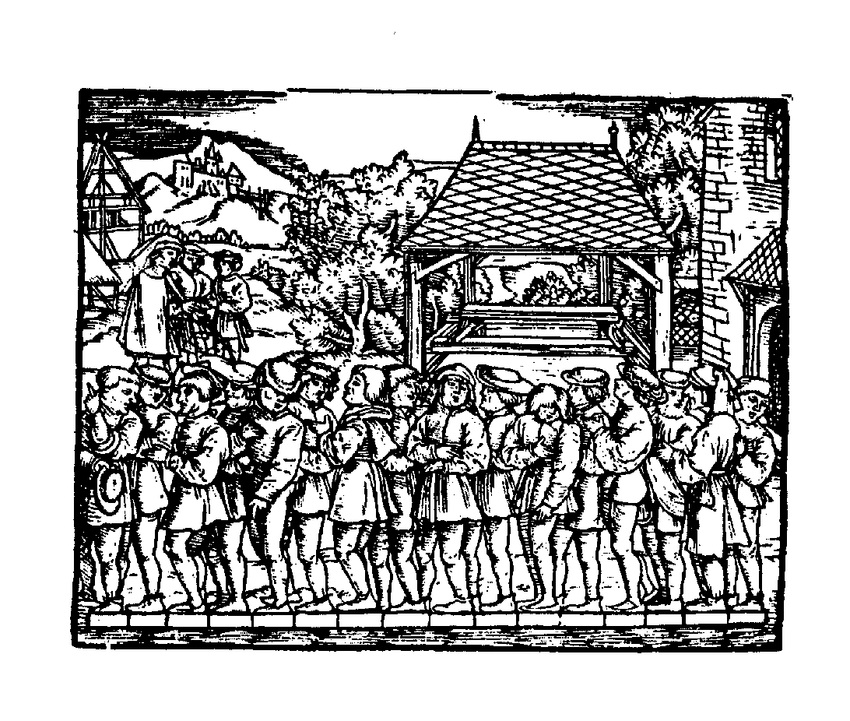
\includegraphics[scale=0.20]{./figs/Rood.png}
    \bigskip

    The determination of a ``right and lawful rood'' or rod in the early sixteenth century in
    Germany by measuring an essentially random selection of 16 men as they leave church
    \footnote{Stephen Stigler (1996). Statistics and the Question of Standards, {\em Journal of Research of
    the National Institute of Standards and Technology}, vol. 101.}.
  \end{center}
\end{frame}
\begin{frame}[fragile] % Measure probability
  \frametitle{The same for chance}

  To measure probability, \pause
  \begin{enumerate}
    \item we first find or make equally probable cases,
    \item then we count.
  \end{enumerate}
  \bigskip \vfill \pause

  The probability of an event $A$, denoted by $\mathbb{P}(A)$, is then
  \begin{align*}
    \mathbb{P}(A) = \frac{\text{no. of cases in which $A$ occurs}}{\text{total no. of cases}}.
  \end{align*}

\end{frame}
\begin{frame}[fragile,t] % Properties of probability
 Now we see that probability has to satisfy the following properties: \pause

 \begin{enumerate}
   \item Probability should be never negative.
   \item If $A$ occurs in all cases, then  $ \mathbb{P}(A)=1$.
   \item If $A$ and $B$ never occur in the same case, then
     \begin{align*}
       \mathbb{P}\left(\text{$A$ or  $B$}\right) = \mathbb{P}(A) + \mathbb{P}(B).
     \end{align*}
 \end{enumerate}
 \vfill \pause

 In particular, the probability of an event not occurring is equal to
 \begin{align*}
   \mathbb{P}(\text{not $A$})  = 1 - \mathbb{P}(A).
 \end{align*}

\end{frame}
\begin{frame}[fragile] % Equi-probable cases
 \begin{center}
   How to generate the equi-probable cases?
 \end{center}
 \vfill \pause
 \begin{center}
   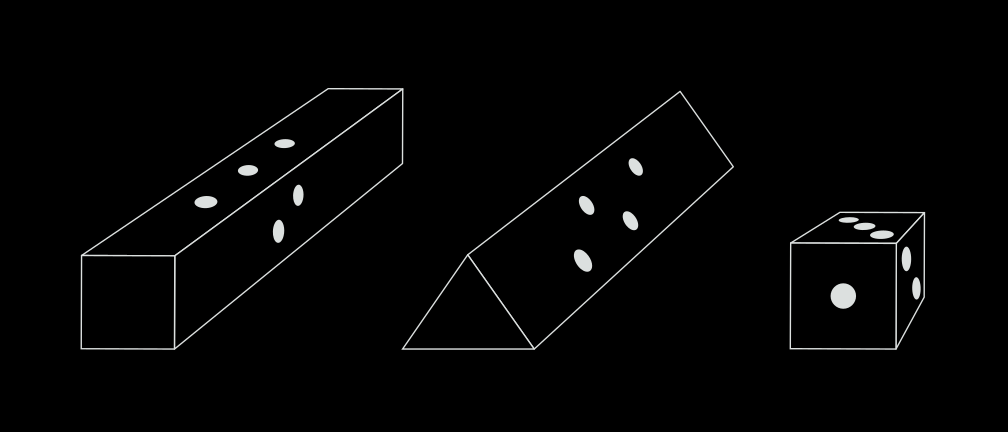
\includegraphics[scale=0.20]{./figs/prism_stick_dice-neg.png}
   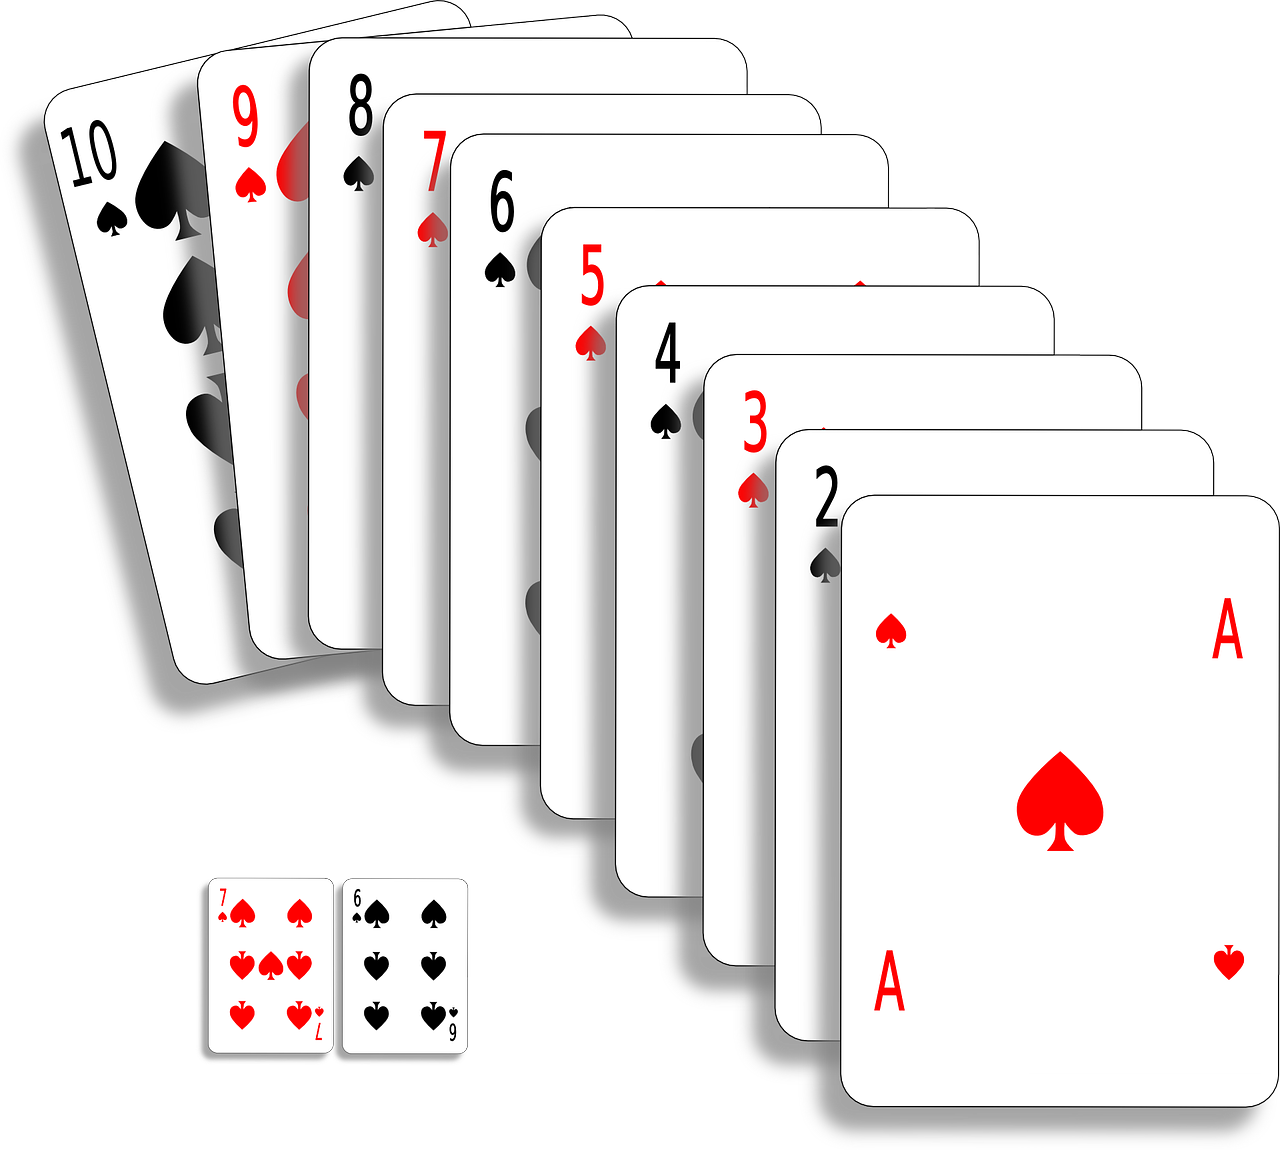
\includegraphics[scale=0.07]{./figs/card-deck.png}
   \bigskip

   Prim sticks (variations of dice) \footnote{Image is from Bennett (1998), {\it Randomness},
   Harvard University Press.} and deck of poker...
 \end{center}
\end{frame}
\begin{frame}[fragile] % Girolamo Cardano
 \begin{center}
   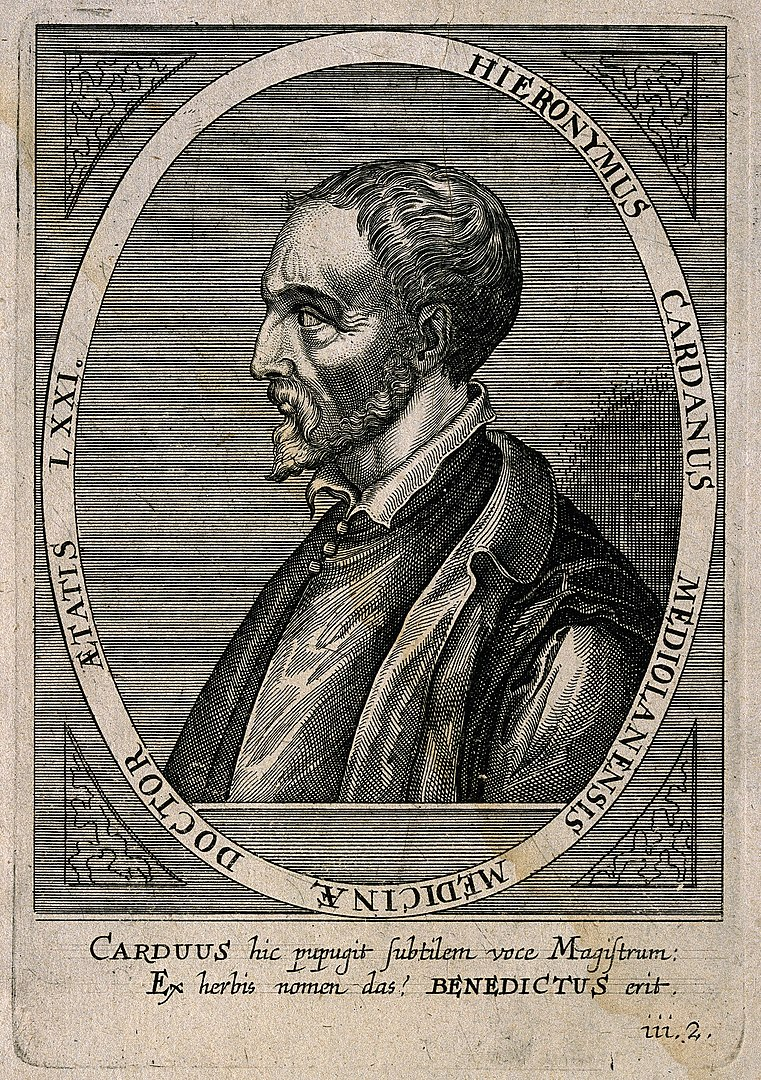
\includegraphics[scale=0.15]{./figs/Girolamo_Cardano.jpg}
   \bigskip

   {\it Girolamo Cardano} (1501 -- 1576),  an Italian polymath, whose interests and proficiencies ranged
   through those of mathematician, physician, biologist, physicist, chemist, astrologer, astronomer,
   philosopher, writer, and gambler. He was one of the most influential mathematicians of the
   Renaissance, and was one of the key figures in the foundation of probability and the earliest
   introducer of the binomial coefficients and the binomial theorem in the Western world.
 \end{center}
\end{frame}
\section{Birthday problem}%
\begin{frame}[fragile,t] % Problem itself
	\frametitle{Birthday Problem}
	{\bf Question:}
  How likely do two students have the same birth day if there are
	\begin{itemize}
		\item 2
		\item 5
		\item 15
		\item 23
		\item 46
		\item 64
		\item 366
	\end{itemize}
	students in the class?
  \vfill \pause

  Assuming that \pause
  \begin{enumerate}
    \item each year has 365 days (i.e., neglecting leap years),
    \item birthdays are equi-probable,
    \item birthdays are independent (no twins in the class).
  \end{enumerate}
\end{frame}
\begin{frame}[fragile,t] % Solving
  \begin{itemize}
    \item Suppose $n=5$.
    \item Let $A$ be the event that there is a shared birthday among these $n$ students.
    % \item Let $\mathbb{P}(A)$ denote the probability that this event $A$ will happen.
    \item It is not easy to compute $\mathbb{P}(A)$ directly.
    \item However, one can compute $\mathbb{P}\left(\text{not $A$}\right)$ by counting: \bigskip
      \begin{center}
        the probability that no two students have the same birthday, or\\
        \bigskip

				all students have different birthday,
			\end{center}
			\bigskip
		\item[] is equal to
			 \begin{align*}
         \mathbb{P}\left(\text{not $A$}\right) = \frac{365}{365} \frac{364}{365} \frac{363}{365} \frac{362}{365} \frac{361}{365}
			\end{align*}
	\item Hence,
		\begin{align*}
      \mathbb{P}(A) = 1 - \mathbb{P}\left(\text{not $A$}\right) = 1- \frac{365}{365} \frac{364}{365} \frac{363}{365} \frac{362}{365} \frac{361}{365}
			\approx 0.027.
		\end{align*}
	\end{itemize}
\end{frame}
\begin{frame}[fragile] % Table and figure
	\begin{align*}
    \mathbb{P}(A) = 1 - \frac{365\times 364 \times\cdots \times(365-n+1)}{365^n}
	\end{align*}

\begin{codes}
% Sage

	n=[2, 5, 15, 23, 64, 366]
	for x in n:
		round(1- gamma(366)/gamma(366-x)/(365^x)*1.0,4)

	for x in range(20):
		print("(",x*5, ",", round(1- gamma(366)/gamma(366-x*5)/(365^(x*5))*1.0,4), ")")

\end{codes}


	\bigskip
	\begin{center}
		\renewcommand{\arraystretch}{1.2}
		\begin{tabular}{|c|c|c|c|c|c|c|c|}
			\hline
			$n$             & \textcolor{gray}{2} & \textcolor{gray}{5} & \textcolor{gray}{15} & \textcolor{gray}{23} & \textcolor{gray}{46} & \textcolor{gray}{64} & \textcolor{gray}{366} \\ \hline
      $\mathbb{P}(A)$ & \only<2->{0.0027}   & \only<3->{0.0271}   & \only<4->{0.2529}    & \only<5->{0.5073}    & \only<6->{0.9483}    & \only<7->{0.9972}    & \only<1->{1.0}        \\ \hline
		\end{tabular}

		\pause
		\bigskip
		\only<8->{
\begin{center}
    \begin{tikzpicture}[scale=0.8, transform shape]
      \begin{axis}[
        axis lines = left,
        xtick={0, 15, 23, 46, 64, 100},
        ytick={0, 0.2529, 0.5073, 0.9483, 0.9972},
        % yticklabels={$0$, $\frac{1}{2\pi}$, $\frac{2 \sqrt{2}}{3\pi}$, $\frac{1}{2}$},
        % legend style={at={(1.0,0.9)},anchor=north},
        % legend style={draw=none},
        % xmin=-8,
        xlabel=$n$,
        ylabel=$\mathbb{P}(A)$,
        xmax=110,
        ymax=1.1,
        ]
        % \addplot[smooth,domain=-9:9,dashed,thin] {0};

        \addplot[domain=-9:9,red,very thick,smooth] coordinates {
          ( 0 , 0.0 )
          ( 5 , 0.0271 )
          ( 10 , 0.1169 )
          ( 15 , 0.2529 )
          ( 20 , 0.4114 )
          ( 25 , 0.5687 )
          ( 30 , 0.7063 )
          ( 35 , 0.8144 )
          ( 40 , 0.8912 )
          ( 45 , 0.941 )
          ( 50 , 0.9704 )
          ( 55 , 0.9863 )
          ( 60 , 0.9941 )
          ( 65 , 0.9977 )
          ( 70 , 0.9992 )
          ( 75 , 0.9997 )
          ( 80 , 0.9999 )
          ( 85 , 1.0 )
          ( 90 , 1.0 )
          ( 95 , 1.0 )
        };
       \def\x{15}
       \def\y{0.2529}
       \addplot[thick, samples=50, smooth,domain=0:101, dashed] coordinates {(\x,0.02) (\x  ,\y)};
       \addplot[thick, samples=50, smooth,domain=0:101, dashed] coordinates {(\x,\y)   (1.50,\y)};
       \def\x{23}
       \def\y{0.5073}
       \addplot[thick, samples=50, smooth,domain=0:101, dashed] coordinates {(\x,0.02) (\x  ,\y)};
       \addplot[thick, samples=50, smooth,domain=0:101, dashed] coordinates {(\x,\y)   (1.50,\y)};
       \def\x{46}
       \def\y{0.9483}
       \addplot[thick, samples=50, smooth,domain=0:101, dashed] coordinates {(\x,0.02) (\x  ,\y)};
       \addplot[thick, samples=50, smooth,domain=0:101, dashed] coordinates {(\x,\y)   (1.50,\y)};
       % \def\x{100}
       % \def\y{1.000}
       % \addplot[thick, samples=50, smooth,domain=0:101, dashed] coordinates {(\x,0.02) (\x  ,\y)};
       % \addplot[thick, samples=50, smooth,domain=0:101, dashed] coordinates {(\x,\y)   (1.50,\y)};
    \end{axis}
    \end{tikzpicture}
  \end{center}
    }
	\end{center}
\end{frame}
\begin{frame}[fragile] % Simulations via Python.
  \begin{center}

 When time permits, we will try some simulations~! \\
 \bigskip

 Source codes are here: \\

 {\tiny\textcolor{gray}{\url{https://github.com/chenle02/2012_Science_Summer_Institute_Auburn_Probability_by_Le}}}
  \end{center}
\end{frame}
\begin{frame}[fragile,t] % COMENTS
  \frametitle{More surprises of this type}
 \begin{enumerate}
   \item Let $C$ be the number of categories (i.e., $C=365$) and $n$ be the number of students. Here
     is one useful approximation:
     \begin{align*}
       \text{when $n=1.2 \sqrt{C}$, the chance of shared something is close to $1/2$.}
     \end{align*}
   \item[] E.g., $1.2\sqrt{365}=22.9$ (Birthday problem), $1.2 \sqrt{60}=9.3$ ({\it Watch problem}). \bigskip
   \item How large should $n$ be to have approximately even probability of a triple birthday match?
   \item[] Answer: 81. \bigskip
   \item Would that be a surprise if you find out with someone, not only you share the same
     birthday, but also the same father's birthday and the same grandfather's birthday?
   \item[]
 \end{enumerate}
\end{frame}
\begin{frame}[fragile] % Matching birthdays with multiple generations.
  \begin{center}
    \renewcommand{\arraystretch}{1.2}
    \begin{tabular}{|c|c|c|c|c|c|} \hline
      Number of generations       & $1$  & $2$              & $3$                & $4$                  & $5$                    \\ \hline
      $n$ to have about even odds & $23$ & \only<2->{$438$} & \only<3->{$8,368$} & \only<4->{$159,870$} & \only<5->{$3,054,312$} \\ \hline
    \end{tabular}

  \end{center}
\end{frame}
\begin{codes}

round(1.2*sqrt(365.0),1)
round(1.2*sqrt(365.0*365.0),1)
round(1.2*sqrt(365.0*365.0*365.0),1)
round(1.2*sqrt(365.0*365.0*365.0*365.0),2)

\end{codes}
\section{Rolling three dices}%
\begin{frame}[fragile] % Questions by Grand Duke
  \frametitle{A question asked by {\it Grand Duke of Tuscany} \\ to {\it Galileo} in early seventh
  century}

  \begin{quotation}
    Three dice are thrown, such as
    \begin{align*}
       9: \: \drawdie[scale=2]{6} \: \drawdie[scale=2]{2} \: \drawdie[scale=2]{1} \\
      10: \: \drawdie[scale=2]{5} \: \drawdie[scale=2]{3} \: \drawdie[scale=2]{2} \\
      11: \: \drawdie[scale=2]{4} \: \drawdie[scale=2]{4} \: \drawdie[scale=2]{3} \\
      12: \: \drawdie[scale=2]{3} \: \drawdie[scale=2]{5} \: \drawdie[scale=2]{4} \\
    \end{align*}
    Counting combinations of numbers, 10 and 11 can be made in 6 ways, as can
    9 and 12. Yet it is known that long observation has made dice-players consider $10$ and  $11$ to
    be more advantageous than  $9$ and $12$. How can this be?
  \end{quotation}
\end{frame}
\begin{frame}[fragile,t] % Dice sums = 9, 10, 11, 12
\begin{minipage}{0.24\textwidth}
  \vspace{7em}
  \begin{center}
    9
  \end{center}
  \begin{align*}
    \drawdie[scale=2]{1} \: \drawdie[scale=2]{2} \: \drawdie[scale=2]{6} \\
    \drawdie[scale=2]{1} \: \drawdie[scale=2]{3} \: \drawdie[scale=2]{5} \\
    \drawdie[scale=2]{1} \: \drawdie[scale=2]{4} \: \drawdie[scale=2]{4} \\
    \drawdie[scale=2]{2} \: \drawdie[scale=2]{2} \: \drawdie[scale=2]{5} \\
    \drawdie[scale=2]{2} \: \drawdie[scale=2]{3} \: \drawdie[scale=2]{4} \\
    \drawdie[scale=2]{3} \: \drawdie[scale=2]{3} \: \drawdie[scale=2]{3} \\
  \end{align*}
\end{minipage}
\begin{minipage}{0.24\textwidth}
  \begin{center}
    10
  \end{center}
  \begin{align*}
    \drawdie[scale=2]{1} \: \drawdie[scale=2]{3} \: \drawdie[scale=2]{6} \\
    \drawdie[scale=2]{1} \: \drawdie[scale=2]{4} \: \drawdie[scale=2]{5} \\
    \drawdie[scale=2]{2} \: \drawdie[scale=2]{2} \: \drawdie[scale=2]{6} \\
    \drawdie[scale=2]{2} \: \drawdie[scale=2]{3} \: \drawdie[scale=2]{5} \\
    \drawdie[scale=2]{2} \: \drawdie[scale=2]{4} \: \drawdie[scale=2]{5} \\
    \drawdie[scale=2]{3} \: \drawdie[scale=2]{3} \: \drawdie[scale=2]{4} \\
  \end{align*}
\end{minipage}
\begin{minipage}{0.24\textwidth}
  \begin{center}
    11
  \end{center}
  \begin{align*}
    \drawdie[scale=2]{1} \: \drawdie[scale=2]{4} \: \drawdie[scale=2]{6} \\
    \drawdie[scale=2]{1} \: \drawdie[scale=2]{5} \: \drawdie[scale=2]{5} \\
    \drawdie[scale=2]{2} \: \drawdie[scale=2]{3} \: \drawdie[scale=2]{6} \\
    \drawdie[scale=2]{2} \: \drawdie[scale=2]{4} \: \drawdie[scale=2]{5} \\
    \drawdie[scale=2]{3} \: \drawdie[scale=2]{3} \: \drawdie[scale=2]{5} \\
    \drawdie[scale=2]{3} \: \drawdie[scale=2]{4} \: \drawdie[scale=2]{4} \\
  \end{align*}
\end{minipage}
\begin{minipage}{0.24\textwidth}
  \vspace{7em}
  \begin{center}
    12
  \end{center}
  \begin{align*}
    \drawdie[scale=2]{1} \: \drawdie[scale=2]{5} \: \drawdie[scale=2]{6} \\
    \drawdie[scale=2]{2} \: \drawdie[scale=2]{4} \: \drawdie[scale=2]{6} \\
    \drawdie[scale=2]{2} \: \drawdie[scale=2]{5} \: \drawdie[scale=2]{5} \\
    \drawdie[scale=2]{3} \: \drawdie[scale=2]{3} \: \drawdie[scale=2]{6} \\
    \drawdie[scale=2]{3} \: \drawdie[scale=2]{4} \: \drawdie[scale=2]{5} \\
    \drawdie[scale=2]{4} \: \drawdie[scale=2]{4} \: \drawdie[scale=2]{4} \\
  \end{align*}
\end{minipage}
\end{frame}
\begin{frame}[fragile,t] % Three dices real
  \begin{align*}
    3  & = \drawdie{1} + \drawdie{1} + \drawdie{1}                                                                                                                                                                                                                   \\
    4  & = \drawdie{1} + \drawdie{1} + \drawdie{2}                                                                                                                                                                                                                   \\
    5  & = \drawdie{1} + \drawdie{1} + \drawdie{3} = \drawdie{1} + \drawdie{2} + \drawdie{2}                                                                                                                                                                         \\
    6  & = \drawdie{1} + \drawdie{1} + \drawdie{4} = \drawdie{1} + \drawdie{2} + \drawdie{3} = \drawdie{2} + \drawdie{2} + \drawdie{2}                                                                                                                               \\
    7  & = \drawdie{1} + \drawdie{1} + \drawdie{5} = \drawdie{1} + \drawdie{2} + \drawdie{4} = \drawdie{2} + \drawdie{2} + \drawdie{3} = \drawdie{3} + \drawdie{3} + \drawdie{1}                                                                                     \\
    8  & = \drawdie{1} + \drawdie{1} + \drawdie{6} = \drawdie{1} + \drawdie{2} + \drawdie{5} = \drawdie{1} + \drawdie{3} + \drawdie{4} = \drawdie{2} + \drawdie{2} + \drawdie{4} = \drawdie{2} + \drawdie{3} + \drawdie{3}                                           \\
    9  & = \drawdie{1} + \drawdie{2} + \drawdie{6} = \drawdie{1} + \drawdie{3} + \drawdie{5} = \drawdie{1} + \drawdie{4} + \drawdie{4} = \drawdie{2} + \drawdie{2} + \drawdie{5} = \drawdie{2} + \drawdie{3} + \drawdie{4} = \drawdie{3} + \drawdie{3} + \drawdie{3} \\
    10 & = \drawdie{1} + \drawdie{3} + \drawdie{6} = \drawdie{1} + \drawdie{4} + \drawdie{5} = \drawdie{2} + \drawdie{2} + \drawdie{6} = \drawdie{2} + \drawdie{3} + \drawdie{5} = \drawdie{2} + \drawdie{4} + \drawdie{5} = \drawdie{3} + \drawdie{3} + \drawdie{4} \\
    11 & = \drawdie{1} + \drawdie{4} + \drawdie{6} = \drawdie{1} + \drawdie{5} + \drawdie{5} = \drawdie{2} + \drawdie{3} + \drawdie{6} = \drawdie{2} + \drawdie{4} + \drawdie{5} = \drawdie{3} + \drawdie{3} + \drawdie{5} = \drawdie{3} + \drawdie{4} + \drawdie{4} \\
    12 & = \drawdie{1} + \drawdie{5} + \drawdie{6} = \drawdie{2} + \drawdie{4} + \drawdie{6} = \drawdie{2} + \drawdie{5} + \drawdie{5} = \drawdie{3} + \drawdie{3} + \drawdie{6} = \drawdie{3} + \drawdie{4} + \drawdie{5} = \drawdie{4} + \drawdie{4} + \drawdie{4} \\
    13 & = \drawdie{1} + \drawdie{6} + \drawdie{6} = \drawdie{2} + \drawdie{5} + \drawdie{6} = \drawdie{3} + \drawdie{4} + \drawdie{6} = \drawdie{3} + \drawdie{5} + \drawdie{5} = \drawdie{4} + \drawdie{4} + \drawdie{5}                                           \\
    14 & = \drawdie{2} + \drawdie{6} + \drawdie{6} = \drawdie{3} + \drawdie{5} + \drawdie{6} = \drawdie{4} + \drawdie{4} + \drawdie{6} = \drawdie{4} + \drawdie{5} + \drawdie{5}                                                                                     \\
    15 & = \drawdie{3} + \drawdie{6} + \drawdie{6} = \drawdie{4} + \drawdie{5} + \drawdie{6} = \drawdie{5} + \drawdie{5} + \drawdie{5}                                                                                                                               \\
    16 & = \drawdie{4} + \drawdie{6} + \drawdie{6} = \drawdie{5} + \drawdie{5} + \drawdie{6}                                                                                                                                                                         \\
    17 & = \drawdie{5} + \drawdie{6} + \drawdie{6}                                                                                                                                                                                                                   \\
    18 & = \drawdie{6} + \drawdie{6} + \drawdie{6}                                                                                                                                                                                                                   \\
  \end{align*}
\end{frame}
\begin{frame}[fragile,t] % Three dices with numbers
 \begin{align*}
    3  & = 1 + 1 + 1                                                             \\
    4  & = 1 + 1 + 2                                                             \\
    5  & = 1 + 1 + 3 = 1 + 2 + 2                                                 \\
    6  & = 1 + 1 + 4 = 1 + 2 + 3 = 2 + 2 + 2                                     \\
    7  & = 1 + 1 + 5 = 1 + 2 + 4 = 2 + 2 + 3 = 3 + 3 + 1                         \\
    8  & = 1 + 1 + 6 = 1 + 2 + 5 = 1 + 3 + 4 = 2 + 2 + 4 = 2 + 3 + 3             \\
    9  & = 1 + 2 + 6 = 1 + 3 + 5 = 1 + 4 + 4 = 2 + 2 + 5 = 2 + 3 + 4 = 3 + 3 + 3 \\
    10 & = 1 + 3 + 6 = 1 + 4 + 5 = 2 + 2 + 6 = 2 + 3 + 5 = 2 + 4 + 4 = 3 + 3 + 4 \\
    11 & = 1 + 4 + 6 = 1 + 5 + 5 = 2 + 3 + 6 = 2 + 4 + 5 = 3 + 3 + 5 = 3 + 4 + 4 \\
    12 & = 1 + 5 + 6 = 2 + 4 + 6 = 2 + 5 + 5 = 3 + 3 + 6 = 3 + 4 + 5 = 4 + 4 + 4 \\
    13 & = 1 + 6 + 6 = 2 + 5 + 6 = 3 + 4 + 6 = 3 + 5 + 5 = 4 + 4 + 5             \\
    14 & = 2 + 6 + 6 = 3 + 5 + 6 = 4 + 4 + 6 = 4 + 5 + 5                         \\
    15 & = 3 + 6 + 6 = 4 + 5 + 6 = 5 + 5 + 5                                     \\
    16 & = 4 + 6 + 6 = 5 + 5 + 6                                                 \\
    17 & = 5 + 6 + 6                                                             \\
    18 & = 6 + 6 + 6
 \end{align*}
\end{frame}
\begin{frame}[fragile,t] % Three dices summary of probabilities

  \begin{center}
  \renewcommand{\arraystretch}{1.2}
  \begin{tabular}{|c|c|c|} \hline
    k  & Probability of a sum of $k$ & $\approx$ \\ \hline
    3  & 1/216                       & 0.5\%     \\
    4  & 3/216                       & 1.4\%     \\
    5  & 6/216                       & 2.8\%     \\
    6  & 10/216                      & 4.6\%     \\
    7  & 15/216                      & 7.0\%     \\
    8  & 21/216                      & 9.7\%     \\
    9  & 25/216                      & 11.6\%    \\
    10 & 27/216                      & 12.5\%    \\
    11 & 27/216                      & 12.5\%    \\
    12 & 25/216                      & 11.6\%    \\
    13 & 21/216                      & 9.7\%     \\
    14 & 15/216                      & 7.0\%     \\
    15 & 10/216                      & 4.6\%     \\
    16 & 6/216                       & 2.8\%     \\
    17 & 3/216                       & 1.4\%     \\
    18 & 1/216                       & 0.5\%     \\ \hline
  \end{tabular}

  \end{center}
\end{frame}
\begin{frame}[fragile,t] % More history of the game

 \begin{center}
   Game of rolling three dices dated back to Roman Empire.
   \bigskip
   \bigskip

   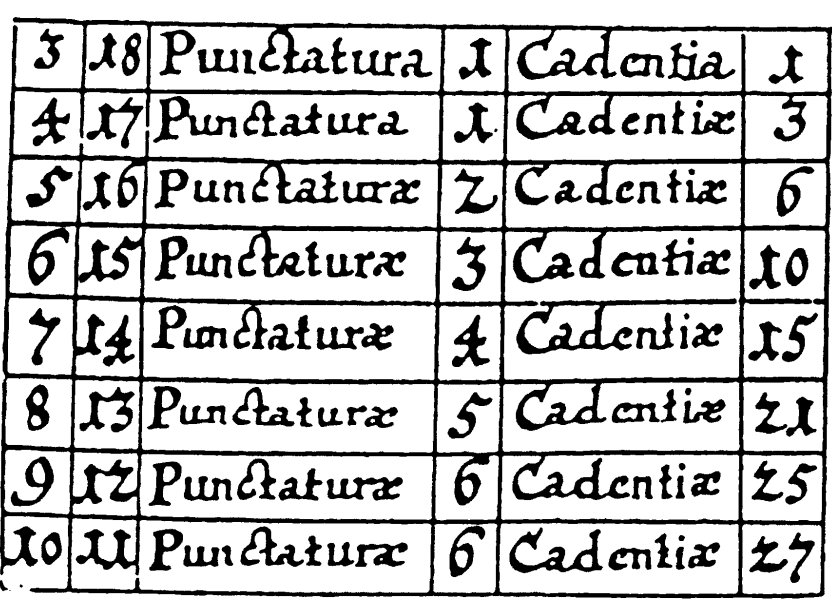
\includegraphics[scale=0.25]{./figs/216cases.png}
   \bigskip

   {\it Richard de Fournival} discovered in 13th century the summary of                                        \\
   216 possible sequences \footnote{Image is from Bennett (1998), {\it Randomness}, Harvard University Press.} \\
   in his poem, \textit{\it De Vetula}, written between 1220 to 1250.


 \end{center}

\end{frame}
\section{Poker}%
\begin{frame}[fragile,t] % Poker -- Hand rankings
\begin{center}
	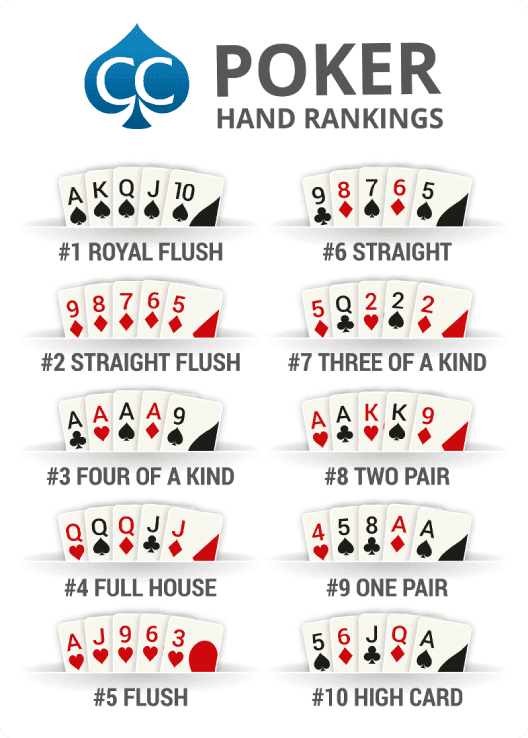
\includegraphics[scale=0.25]{figs/poker-hand-rankings-small.png}
\end{center}
\end{frame}
\begin{frame}[fragile,t] % Probabilities -1
\begin{center}
	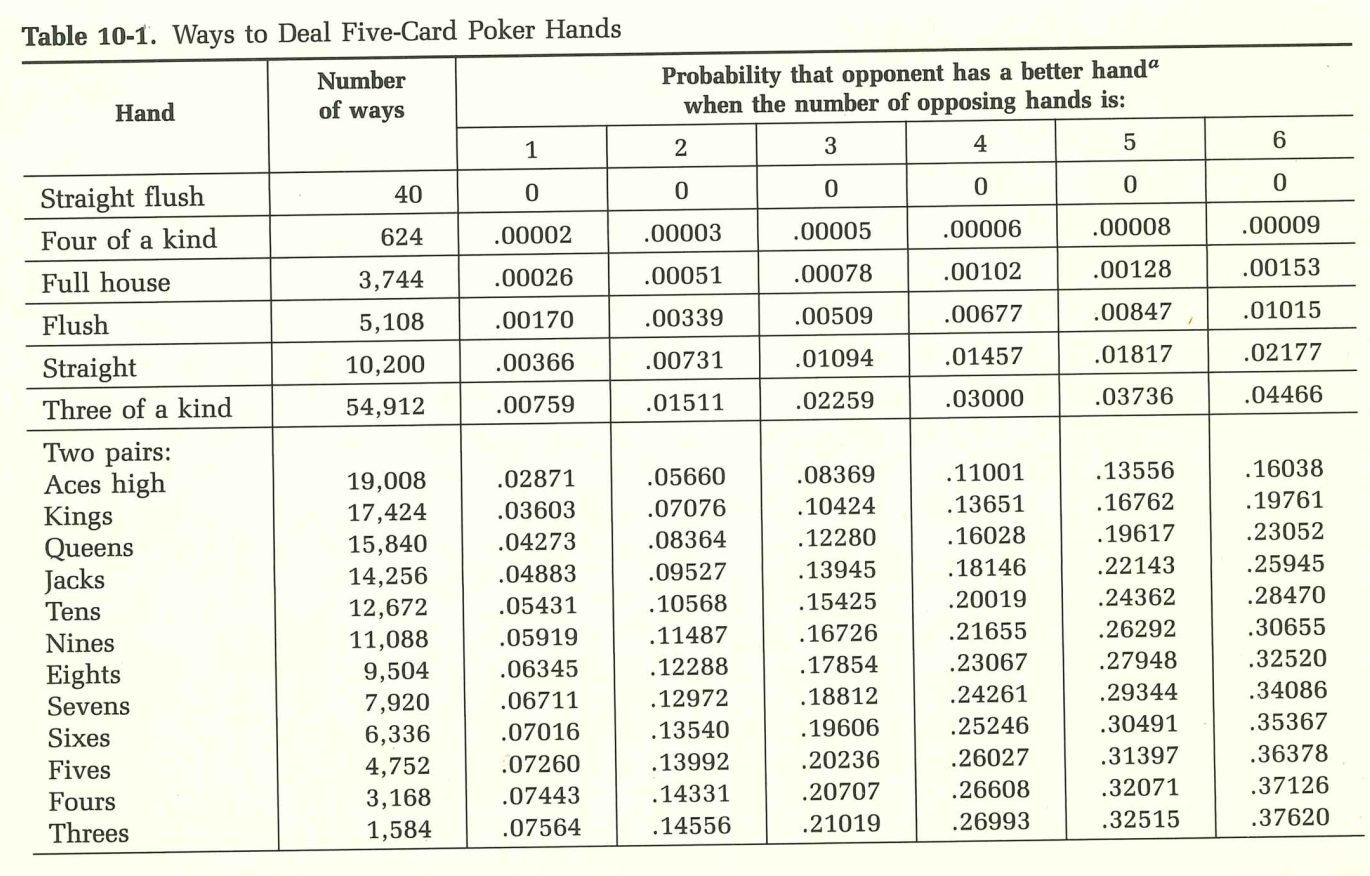
\includegraphics[scale=0.25]{figs/Poker-1.png}
  \footnote{Image from John D. McGervey (1986), {\it Probabilities in everyday life}, Nelson Hall
  Publishers.}
\end{center}
\end{frame}
\begin{frame}[fragile,t] % Probabilities - 2
\begin{center}
	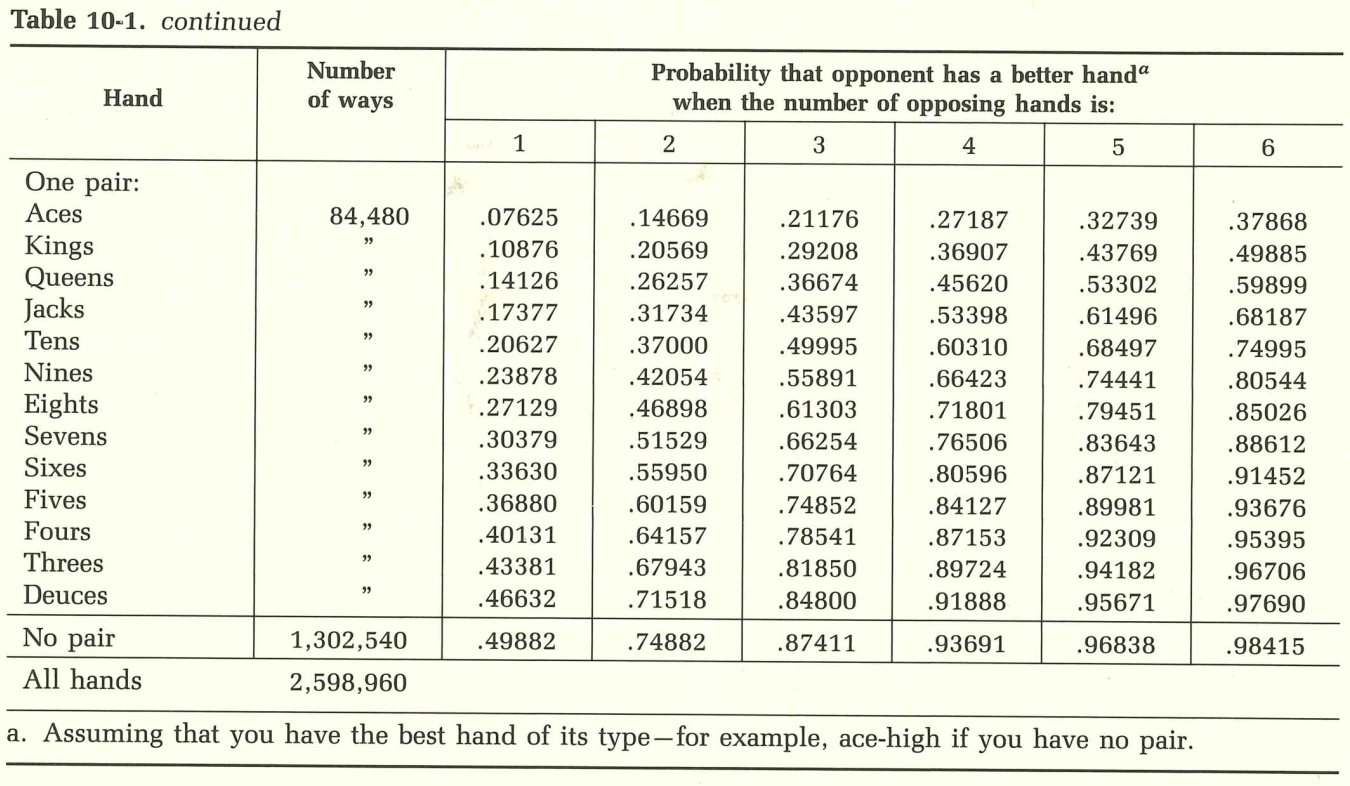
\includegraphics[scale=0.25]{figs/Poker-2.png}
  \footnote{Image from John D. McGervey (1986), {\it Probabilities in everyday life}, Nelson Hall
  Publishers.}
\end{center}
\end{frame}
\begin{frame}<3->[fragile,t] % Thank you and references
  \vfill

 \begin{center}
   \huge

   Thank you for your \\
   listening and participating~!

 \end{center}
 \vfill

 {\noindent \bf References:}\\
 \begin{itemize}
   \item Persi Diaconis and Brian Skyrms (2017). {\it The great ideas about chance.} Princeton
     University Press.
   \item Deborah J. Bennett (1998). {\it Randomness.} Harvard University Press.
   \item John D. McGervey (1986). {\it Probabilities in everyday life}. Nelson Hall Publishers.
 \end{itemize}

\end{frame}
\end{document}
